%\documentclass[10pt]{beamer}
\documentclass[10pt,aspectratio=169]{beamer}
%\documentclass[handout,10pt]{beamer}
%\includeonlyframes{current}
\usepackage{textcomp,colortbl}
\usepackage{amsmath, amssymb, etoolbox, bm, listings}
\usepackage{animate, multirow, hyperref, color, longtable}
\usepackage{makeidx, multicol}
\usepackage[retainorgcmds]{IEEEtrantools}
\hypersetup{
  colorlinks,
  linkcolor=blue,
  urlcolor=blue
}


% These commands are from stack exchange. They are for creating the index of
% examples.
\makeindex
\newenvironment{theindex}
 {\let\item\par
  %definitions for subitem etc
  }{}
\newcommand\indexspace{}

\newcommand{\topic}{01}
\newcommand{\bb}{\mathbb}
\newcommand{\rlang}{\texttt{R} }
\newcommand{\ud}{\,\mathrm{d}}

%\includeonlyframes{current}
\setbeamertemplate{theorems}[numbered]
%\setbeameroption{show notes}
\undef{\example}
\theoremstyle{example}
\newtheorem{example}{\translate{Example}}

\DeclareMathOperator{\var}{var}
\DeclareMathOperator{\cov}{cov}
\DeclareMathOperator{\cor}{cor}
%\DeclareMathOperator{\dp}{dp}
\DeclareMathOperator{\ds}{ds}
\DeclareMathOperator{\dt}{dt}
\DeclareMathOperator{\du}{du}
\DeclareMathOperator{\dv}{dv}
\DeclareMathOperator{\dw}{dw}
\DeclareMathOperator{\dx}{dx}
\DeclareMathOperator{\dA}{dA}
\DeclareMathOperator{\dy}{dy}
\DeclareMathOperator{\dz}{dz}
\DeclareMathOperator{\dr}{dr}
\DeclareMathOperator{\dtheta}{d\theta}
\DeclareMathOperator{\SD}{SD}
\DeclareMathOperator{\Be}{Be}
\DeclareMathOperator{\Bin}{Bin}
\DeclareMathOperator{\Geom}{Geom}
\DeclareMathOperator{\Poi}{Poisson}
\DeclareMathOperator{\Exp}{Exp}

\DeclareMathOperator{\di}{d}
\newcommand{\ddx}{\frac{\di}{\dx}}
\newcommand{\ddz}{\frac{\di}{\dz}}
\newcommand{\ddxt}{\tfrac{\di}{\dx}}
\newcommand{\dydx}{\frac{\dy}{\dx}}
\newcommand{\dydxt}{\tfrac{\dy}{\dx}}
\newcommand{\pdx}[1]{\frac{\partial {#1}}{\partial x}}
\newcommand{\pdy}[1]{\frac{\partial {#1}}{\partial y}}
\newcommand{\rll}[1]{\texttt{#1}}

\usetheme{Boadilla}
\usecolortheme{dove}
%\usetheme[hideallsubsections]{PaloAlto}
% Control the style of bullets:
\setbeamertemplate{enumerate items}[circle]
\setbeamertemplate{section in toc}[circle]
\setbeamercolor{block title}{bg=cyan}
%setbeamercolor{block title}{bg=yellow}
\renewcommand<>\cellcolor[1]{\only#2{\beameroriginal\cellcolor{#1}}}

\setbeamertemplate{footline}[text line]{%
  \parbox{\linewidth}{\vspace*{-8pt}\insertshorttitle\hfill\insertshortauthor\hfill\insertpagenumber}
}
\setbeamertemplate{navigation symbols}{}

\title[]{ Version Control with git}
\author[Topic \topic]{Vik Gopal}
\date{DSA3101 AY 22/23 Sem II}

%\usepackage{Sweave}
\begin{document}
\lstset{
  upquote=true,
  basicstyle=\ttfamily,
  backgroundcolor=\color{yellow!10},
  showstringspaces=false}
\maketitle
\section*{Outline}
\frame{\tableofcontents}

\section{Mental Model}

\begin{frame}{What is git?}
\begin{columns}[T]
\begin{column}{7.5cm}
\begin{center}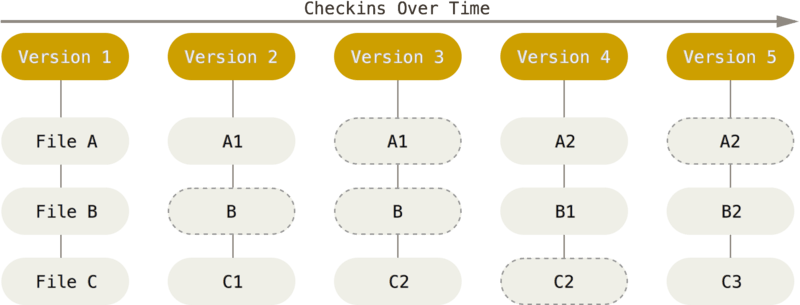
\includegraphics[width=0.8\linewidth]{figs/git-snapshots} \end{center}
\end{column}
\begin{column}{7.5cm}
\begin{center}
\begin{itemize}
\item
  git is a version control software.
\item
  With git, we do not need to worry about keeping track of multiple
  versions of a file or a function.
\item
  We can test new features bravely, without worrying about how to get
  back to an older, working version.
\item
  We can rollback to a previous/alternate version of the code at
  anytime. Nothing is ever lost.
\item
  You can use git on your own, or you can use git as part of a team of
  developers.
\item
  git is distributed.
\item
  \emph{git is not the same as github.} You can use git with or without
  github.
\end{itemize}
\end{center}
\end{column}
\end{columns}
\end{frame}


\begin{frame}{Mental Model}
\begin{columns}[T]
\begin{column}{7.5cm}
\begin{center}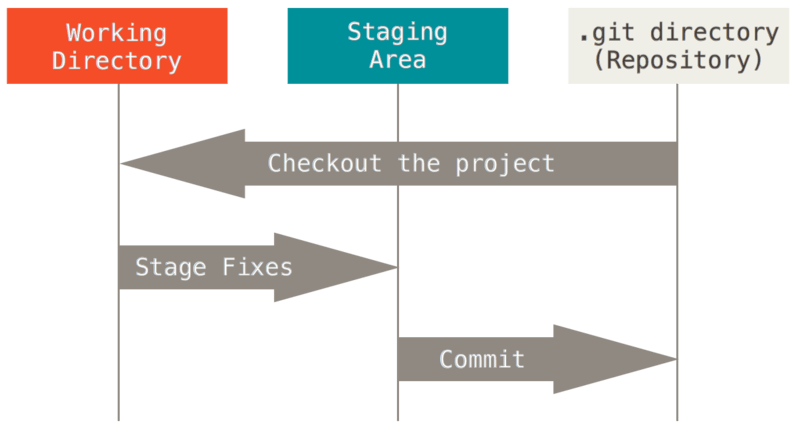
\includegraphics[width=0.85\linewidth]{figs/git-three-areas} 
\end{center}
\end{column}
\begin{column}{7.5cm}
\begin{itemize}
\item
  \emph{Working directory}: A single checkout of one version of the
  project. Also referred to as \emph{working tree}.
\item
  \emph{Staging area}: A temporary, intermediate area that stores
  information about your next commit (version that will be recorded and
  stored). Changes from the working directory need to be
  manually/consciously added to the staging area. The staging area is
  also commonly referred to as the \emph{index}.
\item
  \emph{Repository}: A database of objects (files, meta information,
  commit objects). Changes are not permanent until they have been
  committed.
\end{itemize}
\end{column}
\end{columns}
\end{frame}

\begin{frame}{Mental Model}
\framesubtitle{cont'd}
\begin{columns}[T]
\begin{column}{7.5cm}
\begin{center}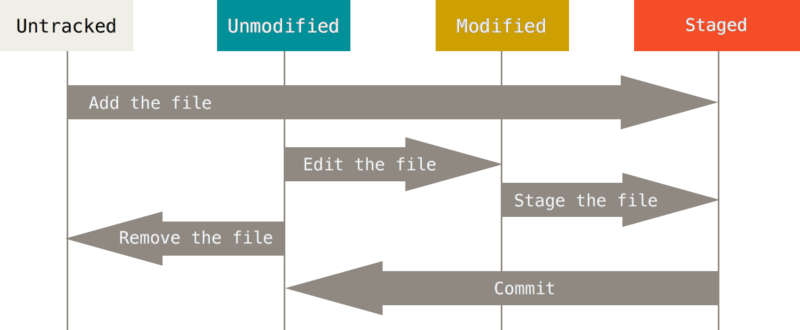
\includegraphics[width=0.8\linewidth]{figs/git-lifecycle} 
\end{center}
\end{column}
\begin{column}{7.5cm}
\begin{itemize}
\item
  A file in our working directory can be either \emph{tracked} or
  \emph{untracked}. A tracked file is something git knows about; we can
  stage and commit it.
\item
  Once tracked, a file is either
  \begin{itemize}
  \item
    unmodified: the same as the file in the latest version of the
    repository.
  \item
    modified: contains changes from the repository version, but not yet
    staged.
  \item
    staged: ready to be committed.
  \end{itemize}
\item
  git does not dictate how, or if at all, you use the staging area. You can
  skip it altogether, every time, if you prefer to work that way.
\end{itemize}
\end{column}
\end{columns}
\end{frame}


\begin{frame}{Terminology}
\begin{columns}[T]
\begin{column}{7.5cm}
\begin{center}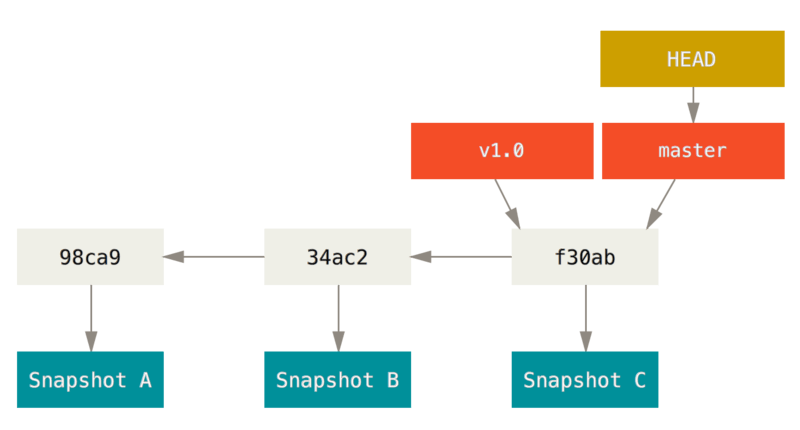
\includegraphics[width=0.75\linewidth]{figs/git-branch-and-history-01} 
\end{center}
\end{column}
\begin{column}{7.5cm}
\begin{itemize}
\item
  Each commit or snapshot is assigned a hash, using SHA-1. This is a
  160-bit checksum.
\item
  In fact, in the object database, every file is named according to its
  SHA-1 hash.
\item
  \texttt{98ca9} commit is the parent of \texttt{34ac2} commit in this
  diagram.
\item
  There is only a single branch in this repository (master).
\item
  HEAD is a special pointer, that keeps track of which branch you are
  currently on.
\begin{itemize}
\item \texttt{HEAD\^} refers to the parent of \texttt{HEAD}.
\item \texttt{HEAD$\sim$2} refers to the grand-parent of \texttt{HEAD}.
\end{itemize}
\item
  v1.0 is a tag; a friendly name for a commit.
\end{itemize}
\end{column}
\end{columns}
\end{frame}

\begin{frame}[plain]{Example Workflow (Forward)}
\begin{center}
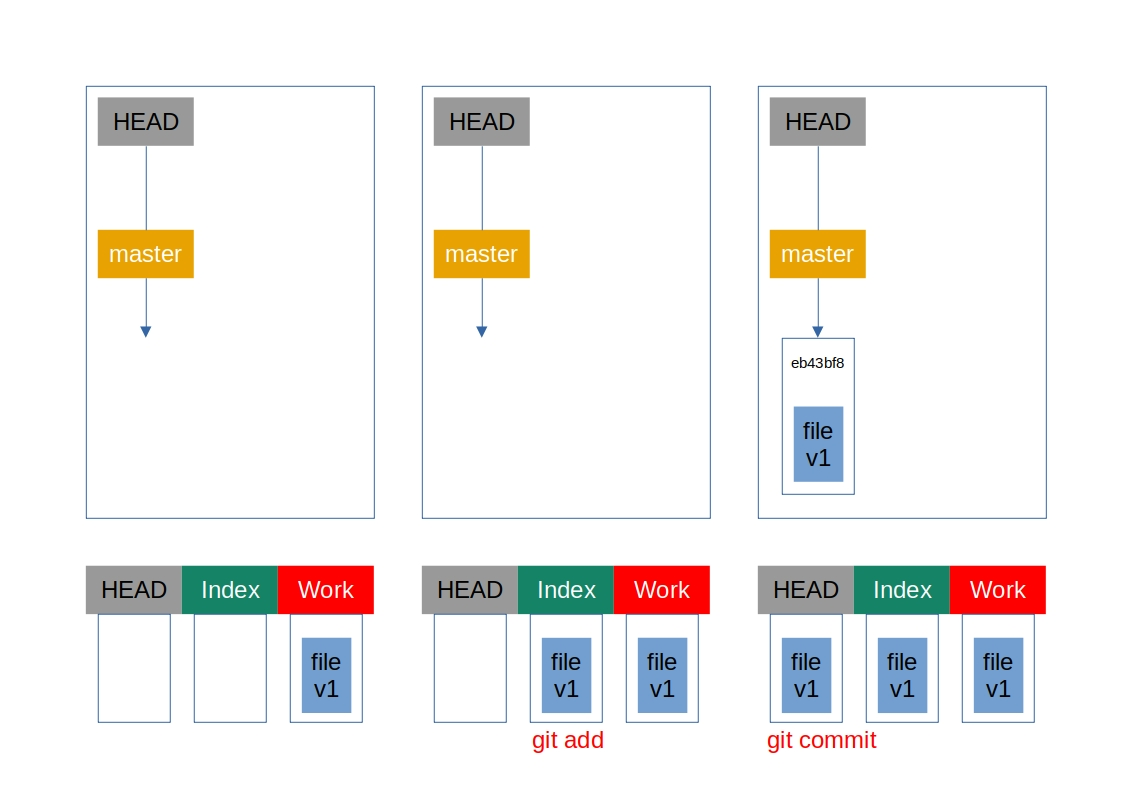
\includegraphics[width=0.7\linewidth]{figs/git_workflow_02a} 
\end{center}
\end{frame}

\begin{frame}[plain]{Example Workflow (Forward)}
\begin{center}
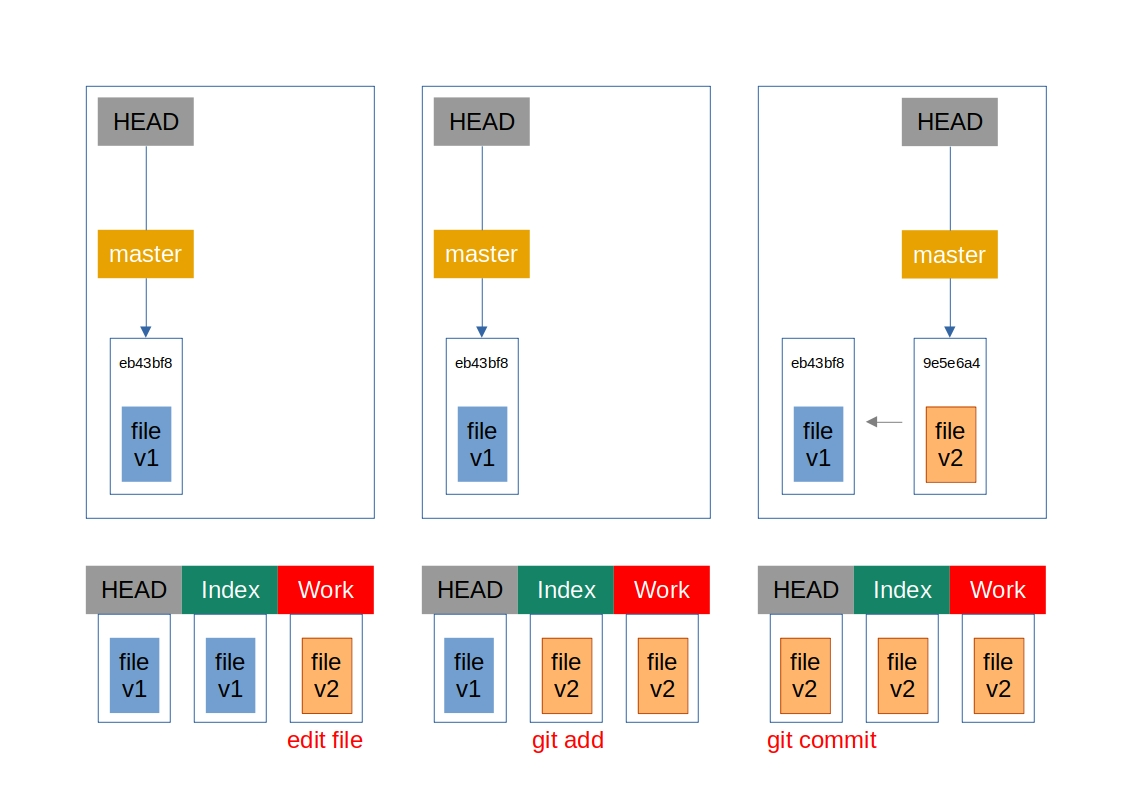
\includegraphics[width=0.7\linewidth]{figs/git_workflow_02b} 
\end{center}
\end{frame}

\begin{frame}[fragile]{Common Commands}
\begin{columns}[T]
\begin{column}{7.5cm}
\begin{itemize}
\item
  \texttt{git\ add}, \texttt{git\ commit}
\item
  \texttt{git\ diff}, \texttt{git\ log}, \texttt{git\ show},
  \texttt{git\ blame}
\item
  \texttt{git\ checkout}, \texttt{git\ switch}, \texttt{git\ branch}
\item
  \texttt{git\ reset}, \texttt{git\ restore}
\item
  \texttt{git\ push}, \texttt{git\ pull}, \texttt{git\ fetch},
  \texttt{git\ remote}
\item
  \texttt{git\ merge}, \texttt{git\ rebase}
\end{itemize}
\end{column}
\begin{column}{7.5cm}
\begin{block}{Help!}
To get help on any of these commands, run it the command with the
\texttt{help} option. For instance:
\begin{lstlisting}
$ git log --help
\end{lstlisting}

\end{block}
\end{column}
\end{columns}

\end{frame}

\begin{frame}[fragile]{Common Commands}
\framesubtitle{cont'd}
\begin{itemize}
\item Checking on the current situation:
\begin{lstlisting}
$ git status


On branch master
Changes to be committed:
Your branch is up to date with 'origin/master'.
  (use "git restore --staged <file>..." to unstage)

	modified:   file1
	modified:   file2
	modified:   file3
\end{lstlisting}
\end{itemize}
\end{frame}

\begin{frame}[fragile,shrink=16]{Common Commands}
\framesubtitle{cont'd}
\begin{itemize}
\item Displaying the difference between files
\begin{lstlisting}
$ git diff


diff --git a/CONTRIBUTING.md b/CONTRIBUTING.md
index 8ebb991..643e24f 100644
--- a/CONTRIBUTING.md
+++ b/CONTRIBUTING.md
@@ -65,7 +65,8 @@ branch directly, things can get messy.
 Please include a nice description of your changes when you submit your PR;
 if we have to read the whole diff to figure out why you're contributing
 in the first place, you're less likely to get feedback and have your change
-merged in.
+merged in. Also, split your changes into comprehensive chunks if your patch is
+longer than a dozen lines.

 If you are starting to work on a particular area, feel free to submit a PR
 that highlights your work in progress (and note in the PR title that it's
\end{lstlisting}
\end{itemize}
\end{frame}

\begin{frame}[fragile]{Common Commands}
\framesubtitle{cont'd}
\begin{itemize}
\item Exploring history
\begin{lstlisting}
$ git log --stat


commit ca82a6dff817ec66f44342007202690a93763949
Author: Scott Chacon <schacon@gee-mail.com>
Date:   Mon Mar 17 21:52:11 2008 -0700

    Change version number

 Rakefile | 2 +-
 1 file changed, 1 insertion(+), 1 deletion(-)
\end{lstlisting}
\end{itemize}
\end{frame}

\section{Branching}
\frame{\tableofcontents[currentsection]}

\begin{frame}{Git Branching}
\begin{center}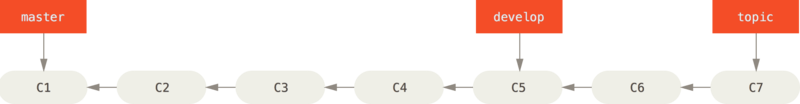
\includegraphics[width=0.6\linewidth]{figs/git-lr-branches-1} \end{center}

\begin{center}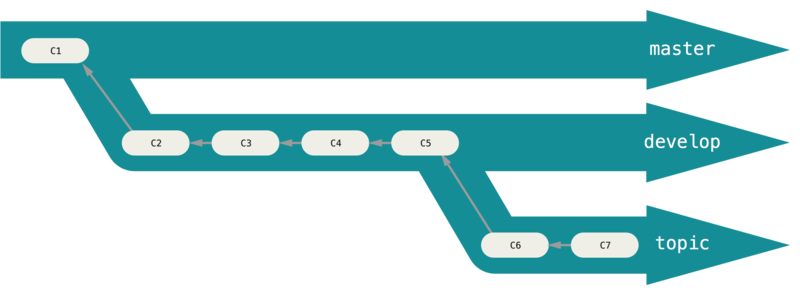
\includegraphics[width=0.6\linewidth]{figs/git-lr-branches-2} \end{center}
\end{frame}

\begin{frame}{Git Branching}
\framesubtitle{cont'd}
\begin{itemize}
\item
  To test out new features/debug things, we can create new branches.
\item
  In git, this is fast and lightweight.
\item
  There are three branches here: \texttt{develop} is ahead of
  \texttt{master}, and \texttt{topic} is further ahead of
  \texttt{develop}.
\item
  We can work on experimental new features in \texttt{develop}, while
  the main codebase in \texttt{master} remains stable in production.
\end{itemize}
\end{frame}

\begin{frame}[plain]{Local Branches}
\begin{center}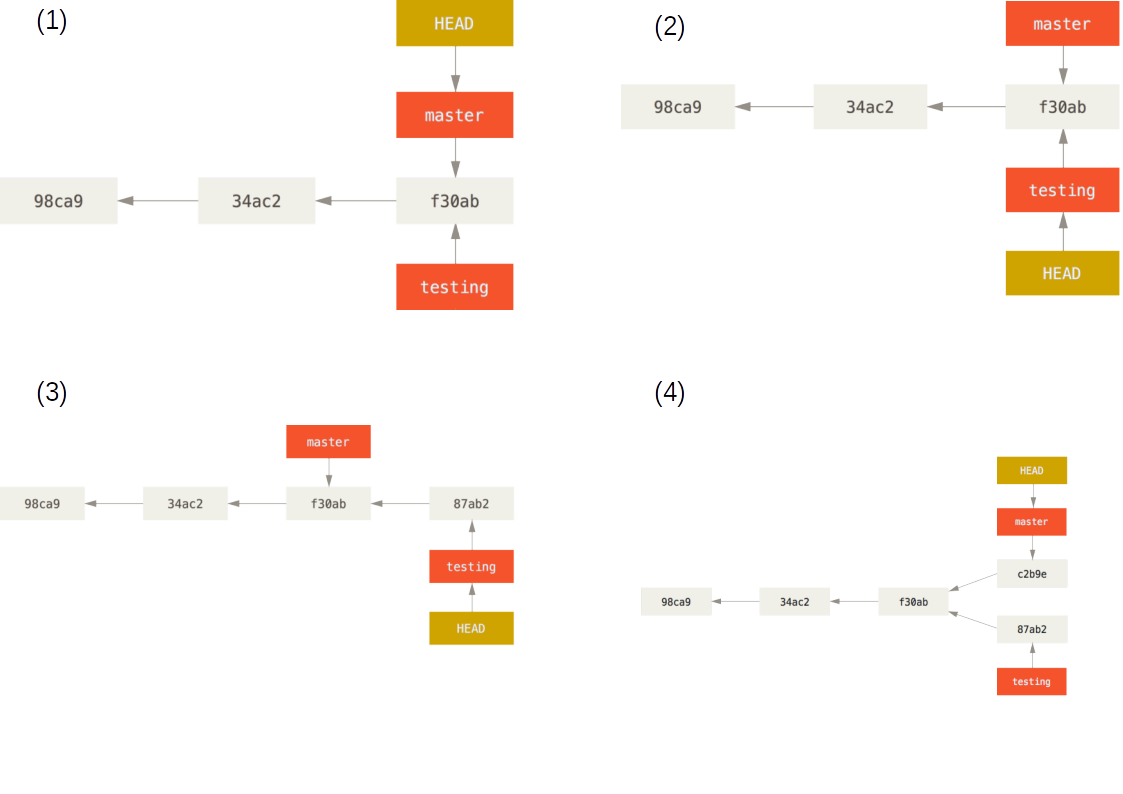
\includegraphics[width=0.75\linewidth]{figs/branching_seq_01} \end{center}
\end{frame}

\begin{frame}[plain]{Remote Branches}
\begin{center}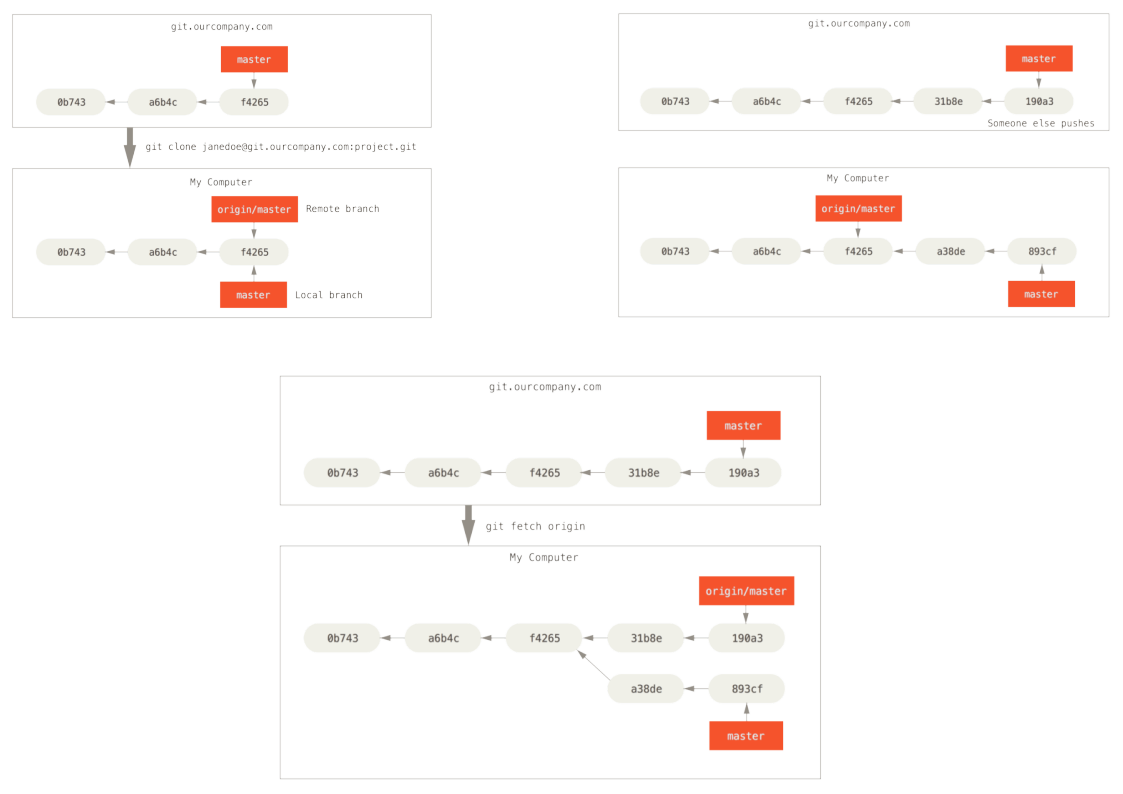
\includegraphics[width=0.75\linewidth]{figs/branching_seq_02} 
\end{center}
\end{frame}

\begin{frame}[plain]{Integrating Changes}
\begin{center}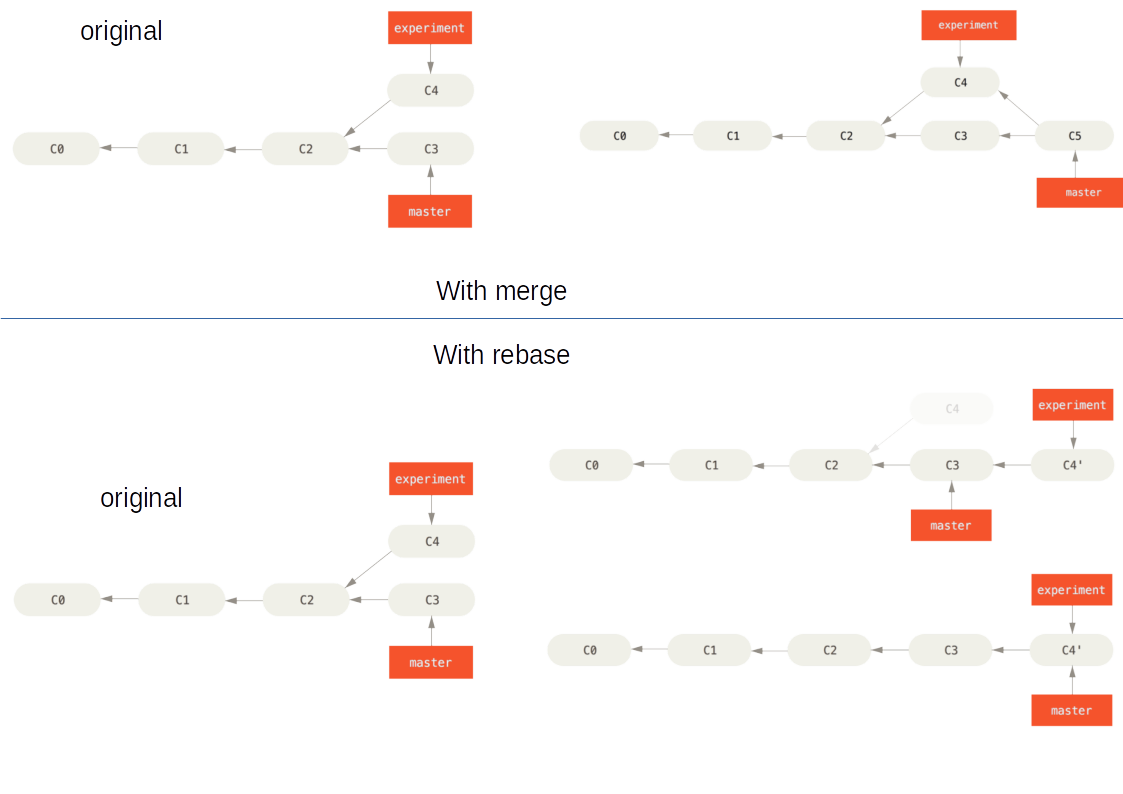
\includegraphics[width=0.75\linewidth]{figs/rebase_example} 
\end{center}
\end{frame}

\begin{frame}[fragile]{Common Workflows}
\begin{itemize}
\item Individual developer:
\begin{lstlisting}
$ git switch -c alsa-audio
$ # edit/compile/test
$ git restore curses/ux_audio_oss.c 
$ git add curses/ux_audio_alsa.c
$ # edit/compile/test
$ git diff HEAD (4)
$ git commit -a -s 
$ # edit/compile/test
$ git diff HEAD^
$ git commit -a --amend 
$ git switch master 
$ git merge alsa-audio 
$ git log --since='3 days ago' 
$ git log v2.43.. curses/ 
\end{lstlisting}
\end{itemize}
\end{frame}

\begin{frame}[fragile]{Common Workflows}
\begin{itemize}
\item Participant developer:
\begin{lstlisting}
$ git clone git://git.kernel.org/pub/scm/.../torvalds/linux-2.6 my2.6
$ cd my2.6
$ git switch -c mine master 
$ # edit/compile/test; 
$ git commit -a -s 
$ git switch master 
$ git pull origin
$ git merge mine
\end{lstlisting}
\end{itemize}
\end{frame}

\begin{frame}[plain]{Common Distributed Workflows}
\begin{center}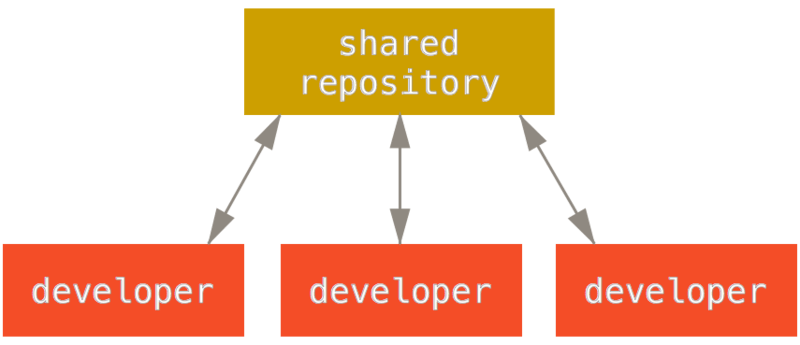
\includegraphics[width=0.75\linewidth]{figs/centralized_workflow} 
\end{center}
\end{frame}

\begin{frame}[plain]{Common Distributed Workflows}
\framesubtitle{cont'd}
\begin{center}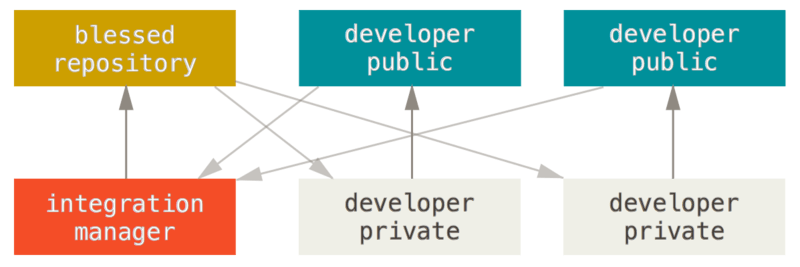
\includegraphics[width=0.75\linewidth]{figs/integration-manager} 
\end{center}
\end{frame}

\section{Miscellaneous}
\frame{\tableofcontents[currentsection]}

\begin{frame}{Ignoring Files}
\begin{itemize}
\item
  The \texttt{.gitignore} file contains patterns that let git know which
  files should intentionally not be tracked.
\item
  A separator \texttt{/} at the end of a line indicates that it is a
  folder that should be ignored.
\end{itemize}
\begin{block}{Examples}
\begin{enumerate}
\def\labelenumi{\arabic{enumi}.}
\item
  \texttt{hello.*} matches any file or directory that begins with
  \texttt{hello.}
\item
  \texttt{/hello.*} matches \texttt{hello.R} but not
  \texttt{dir1/hello.R} (pattern restricted to only this directory).
\item
  \texttt{foo/} will match a directory and everything under it, but not
  any file named \texttt{foo}.
\item
  \texttt{foo/*} will match any files under the directory \texttt{foo},
  but not \texttt{foo/bar/hello.R}. The asterisk does not match the
  \texttt{/} separator character.
\end{enumerate}
\end{block}
\end{frame}

\begin{frame}{Using Staging}
\begin{enumerate}
\def\labelenumi{\arabic{enumi}.}
\item
  When working, I frequently make small changes and test them. Each time
  a small change is working, I stage it so that my working tree is
  clean. Now \texttt{git\ diff} will only highlight the next small
  change I am working on.
\item
  Sometimes, I have made many changes to many files without committing
  or staging. Committing them at one go would not be meaningful. With
  the staging area, I can stage and commit the changes (even partial
  file changes) one group at a time.
\item
  If you do not feel this is how you would like to work, feel free to
  use

\begin{itemize}
\item
  \texttt{git\ status\ -s}
\item
  \texttt{git\ commit\ -a} 
\item The latter command will automatically stage
  and then commit the modified files in your working tree. \emph{This
  skips the staging area.}
\end{itemize}
\end{enumerate}

\end{frame}


\begin{frame}{git Command Line}
\begin{itemize}
\item
  The git command line works from the git-bash shell.
  \begin{itemize}
  \item
    Full documentation for every command is accessible through
    \texttt{git\ \textless{}command\_name\textgreater{}\ -\/-help}.
  \end{itemize}
\item
  Several commands can take revisions, and file paths as input.
  \begin{itemize}
  \item
    A revision can be a commit, branch or a tag
  \end{itemize}
\item
  Revisions and file paths can be separated using \texttt{-\/-}
\end{itemize}

\begin{block}{Examples}
\begin{itemize}
\item
  \texttt{git\ show\ abde09}
  \begin{itemize}
  \item
    Provides details about commit that begins with abde09.
  \end{itemize}
\item
  \texttt{git\ show\ abde09\ -\/-\ test.sql}
  \begin{itemize}
  \item
    Provides details about file test.sql in commit that begins with
    abde09.
  \end{itemize}
\item
  \texttt{git\ diff\ 6c05cfc..b1ab8f7\ \ -\/-\ src/01\_git\_workshop.Rmd}
  \begin{itemize}
  \item
    Shows differences between file \texttt{src/01\_git\_workshop.Rmd}
    between older commit \texttt{6c05cfc} and newer commit
    \texttt{b1ab8f7}.
  \end{itemize}
\end{itemize}
\end{block}
\end{frame}

\section{References}
\frame{\tableofcontents[currentsection]}

% Other commands
% Summary

\begin{frame}{Other Useful git Commands}
\begin{itemize}
\item \texttt{git bisect}, \texttt{git blame}
\item \texttt{git rebase}
\item \texttt{git log -S}
\item \texttt{git grep}
\end{itemize}
\end{frame}


\begin{frame}{Using github in DSA3101 Projects}
\begin{itemize}
\item Create pull requests and tag your team-mate to review the code.
\item As a reviewer, read, run and suggest improvements.
\item Create topic branches, not individually named branches.
\item Use the project management features to track issues and tasks.
\item Use the webpage to document your model or API.
\end{itemize}
\end{frame}

\begin{frame}{Help!}
\begin{columns}
\begin{column}{7.5cm}
\begin{enumerate}
\def\labelenumi{\arabic{enumi}.}
\item
  The \href{https://www.git-scm.com/}{git website}.
\item
  A very neat
  \href{https://ndpsoftware.com/git-cheatsheet.html}{interactive
  visualisation}
\item
  On \href{http://www-cs-students.stanford.edu/~blynn/gitmagic/}{the
  magic of git}.
\item
  Github \href{https://docs.github.com/en}{documentation pages}.
\end{enumerate}
\end{column}
%\onslide<2>
\begin{column}{7.5cm}
\begin{enumerate}
\def\labelenumi{\arabic{enumi}.}
\item
  Use it for your own single-person projects.
\item
  Use it in school projects.
\end{enumerate}

Do not be afraid of ``breaking'' things. With git, it is almost
\emph{always} possible to recover.

\end{column}
\end{columns}
\end{frame}

\end{document}
